\documentclass[12pt,]{article}
\usepackage{lmodern}
\usepackage{amssymb,amsmath}
\usepackage{ifxetex,ifluatex}
\usepackage{fixltx2e} % provides \textsubscript
\ifnum 0\ifxetex 1\fi\ifluatex 1\fi=0 % if pdftex
  \usepackage[T1]{fontenc}
  \usepackage[utf8]{inputenc}
\else % if luatex or xelatex
  \ifxetex
    \usepackage{mathspec}
  \else
    \usepackage{fontspec}
  \fi
  \defaultfontfeatures{Ligatures=TeX,Scale=MatchLowercase}
\fi
% use upquote if available, for straight quotes in verbatim environments
\IfFileExists{upquote.sty}{\usepackage{upquote}}{}
% use microtype if available
\IfFileExists{microtype.sty}{%
\usepackage{microtype}
\UseMicrotypeSet[protrusion]{basicmath} % disable protrusion for tt fonts
}{}
\usepackage[margin=1in]{geometry}
\usepackage{hyperref}
\hypersetup{unicode=true,
            pdftitle={Coursework 1},
            pdfauthor={Jennifer J. Stiens},
            pdfborder={0 0 0},
            breaklinks=true}
\urlstyle{same}  % don't use monospace font for urls
\usepackage{color}
\usepackage{fancyvrb}
\newcommand{\VerbBar}{|}
\newcommand{\VERB}{\Verb[commandchars=\\\{\}]}
\DefineVerbatimEnvironment{Highlighting}{Verbatim}{commandchars=\\\{\}}
% Add ',fontsize=\small' for more characters per line
\usepackage{framed}
\definecolor{shadecolor}{RGB}{248,248,248}
\newenvironment{Shaded}{\begin{snugshade}}{\end{snugshade}}
\newcommand{\KeywordTok}[1]{\textcolor[rgb]{0.13,0.29,0.53}{\textbf{#1}}}
\newcommand{\DataTypeTok}[1]{\textcolor[rgb]{0.13,0.29,0.53}{#1}}
\newcommand{\DecValTok}[1]{\textcolor[rgb]{0.00,0.00,0.81}{#1}}
\newcommand{\BaseNTok}[1]{\textcolor[rgb]{0.00,0.00,0.81}{#1}}
\newcommand{\FloatTok}[1]{\textcolor[rgb]{0.00,0.00,0.81}{#1}}
\newcommand{\ConstantTok}[1]{\textcolor[rgb]{0.00,0.00,0.00}{#1}}
\newcommand{\CharTok}[1]{\textcolor[rgb]{0.31,0.60,0.02}{#1}}
\newcommand{\SpecialCharTok}[1]{\textcolor[rgb]{0.00,0.00,0.00}{#1}}
\newcommand{\StringTok}[1]{\textcolor[rgb]{0.31,0.60,0.02}{#1}}
\newcommand{\VerbatimStringTok}[1]{\textcolor[rgb]{0.31,0.60,0.02}{#1}}
\newcommand{\SpecialStringTok}[1]{\textcolor[rgb]{0.31,0.60,0.02}{#1}}
\newcommand{\ImportTok}[1]{#1}
\newcommand{\CommentTok}[1]{\textcolor[rgb]{0.56,0.35,0.01}{\textit{#1}}}
\newcommand{\DocumentationTok}[1]{\textcolor[rgb]{0.56,0.35,0.01}{\textbf{\textit{#1}}}}
\newcommand{\AnnotationTok}[1]{\textcolor[rgb]{0.56,0.35,0.01}{\textbf{\textit{#1}}}}
\newcommand{\CommentVarTok}[1]{\textcolor[rgb]{0.56,0.35,0.01}{\textbf{\textit{#1}}}}
\newcommand{\OtherTok}[1]{\textcolor[rgb]{0.56,0.35,0.01}{#1}}
\newcommand{\FunctionTok}[1]{\textcolor[rgb]{0.00,0.00,0.00}{#1}}
\newcommand{\VariableTok}[1]{\textcolor[rgb]{0.00,0.00,0.00}{#1}}
\newcommand{\ControlFlowTok}[1]{\textcolor[rgb]{0.13,0.29,0.53}{\textbf{#1}}}
\newcommand{\OperatorTok}[1]{\textcolor[rgb]{0.81,0.36,0.00}{\textbf{#1}}}
\newcommand{\BuiltInTok}[1]{#1}
\newcommand{\ExtensionTok}[1]{#1}
\newcommand{\PreprocessorTok}[1]{\textcolor[rgb]{0.56,0.35,0.01}{\textit{#1}}}
\newcommand{\AttributeTok}[1]{\textcolor[rgb]{0.77,0.63,0.00}{#1}}
\newcommand{\RegionMarkerTok}[1]{#1}
\newcommand{\InformationTok}[1]{\textcolor[rgb]{0.56,0.35,0.01}{\textbf{\textit{#1}}}}
\newcommand{\WarningTok}[1]{\textcolor[rgb]{0.56,0.35,0.01}{\textbf{\textit{#1}}}}
\newcommand{\AlertTok}[1]{\textcolor[rgb]{0.94,0.16,0.16}{#1}}
\newcommand{\ErrorTok}[1]{\textcolor[rgb]{0.64,0.00,0.00}{\textbf{#1}}}
\newcommand{\NormalTok}[1]{#1}
\usepackage{longtable,booktabs}
\usepackage{graphicx,grffile}
\makeatletter
\def\maxwidth{\ifdim\Gin@nat@width>\linewidth\linewidth\else\Gin@nat@width\fi}
\def\maxheight{\ifdim\Gin@nat@height>\textheight\textheight\else\Gin@nat@height\fi}
\makeatother
% Scale images if necessary, so that they will not overflow the page
% margins by default, and it is still possible to overwrite the defaults
% using explicit options in \includegraphics[width, height, ...]{}
\setkeys{Gin}{width=\maxwidth,height=\maxheight,keepaspectratio}
\IfFileExists{parskip.sty}{%
\usepackage{parskip}
}{% else
\setlength{\parindent}{0pt}
\setlength{\parskip}{6pt plus 2pt minus 1pt}
}
\setlength{\emergencystretch}{3em}  % prevent overfull lines
\providecommand{\tightlist}{%
  \setlength{\itemsep}{0pt}\setlength{\parskip}{0pt}}
\setcounter{secnumdepth}{0}
% Redefines (sub)paragraphs to behave more like sections
\ifx\paragraph\undefined\else
\let\oldparagraph\paragraph
\renewcommand{\paragraph}[1]{\oldparagraph{#1}\mbox{}}
\fi
\ifx\subparagraph\undefined\else
\let\oldsubparagraph\subparagraph
\renewcommand{\subparagraph}[1]{\oldsubparagraph{#1}\mbox{}}
\fi

%%% Use protect on footnotes to avoid problems with footnotes in titles
\let\rmarkdownfootnote\footnote%
\def\footnote{\protect\rmarkdownfootnote}

%%% Change title format to be more compact
\usepackage{titling}

% Create subtitle command for use in maketitle
\newcommand{\subtitle}[1]{
  \posttitle{
    \begin{center}\large#1\end{center}
    }
}

\setlength{\droptitle}{-2em}

  \title{Coursework 1}
    \pretitle{\vspace{\droptitle}\centering\huge}
  \posttitle{\par}
    \author{Jennifer J. Stiens}
    \preauthor{\centering\large\emph}
  \postauthor{\par}
    \date{}
    \predate{}\postdate{}
  

\begin{document}
\maketitle

\href{mailto:j.j.stiens@gmail.com}{\nolinkurl{j.j.stiens@gmail.com}}

\href{https://github.com/jenjane118/ngs_tutorials}{github.com/jenjane118/ngs\_tutorials}

\subsection{Question 1}\label{question-1}

\emph{Using good NGS practices, remap Negative.fq so that the mapping
statistics improve.}

\emph{a) View file and work out what is wrong with reads. Generate
fastqc report.}

First I will generate a Fastqc report of the trimmed\_Negative.fq
sequence file.

\begin{Shaded}
\begin{Highlighting}[]
\ExtensionTok{/s/software/fastqc/v0.11.8/FastQC/fastqc}\NormalTok{ trimmed_Negative.fq}
\end{Highlighting}
\end{Shaded}

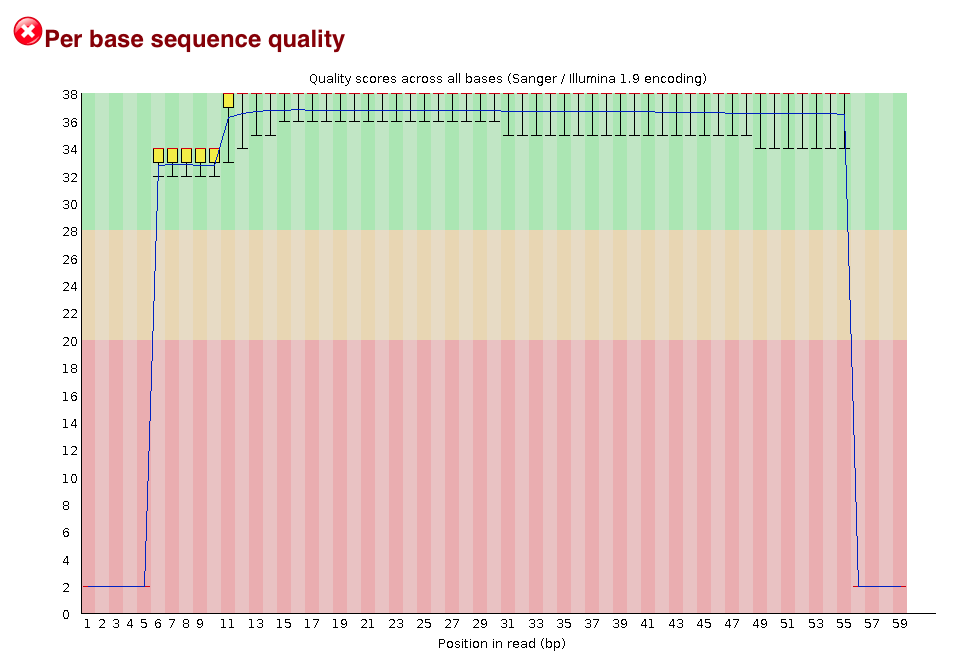
\includegraphics{trimmed_Negative_fastqc.png}\\
\href{/d/projects/u/sj003/course_materials/fastq/coursework_1/trimmed_Negative_fastqc.html}{fastqc
report original}

This shows very low sequence quality at the start and end of each read.
Looking at the fasta file on the shell screen, it is obvious that the
reads have 5 N's at the 5' end and 4 N's at the 3' end of each read that
need to be removed. To do this, we use cutadapt to process each read.

\begin{Shaded}
\begin{Highlighting}[]
\ExtensionTok{/s/software/anaconda/python3/bin/cutadapt}\NormalTok{ --trim-n -o trimmedNs_negative.fq trimmed_Negative.fq}
\FunctionTok{less}\NormalTok{ trimmedNs_negative.fq}
\end{Highlighting}
\end{Shaded}

Running Fastqc again, you can see an improvement in the sequence
quality.

\begin{Shaded}
\begin{Highlighting}[]
\ExtensionTok{/s/software/fastqc/v0.11.8/FastQC/fastqc}\NormalTok{ trimmedNs_Negative.fq}
\end{Highlighting}
\end{Shaded}

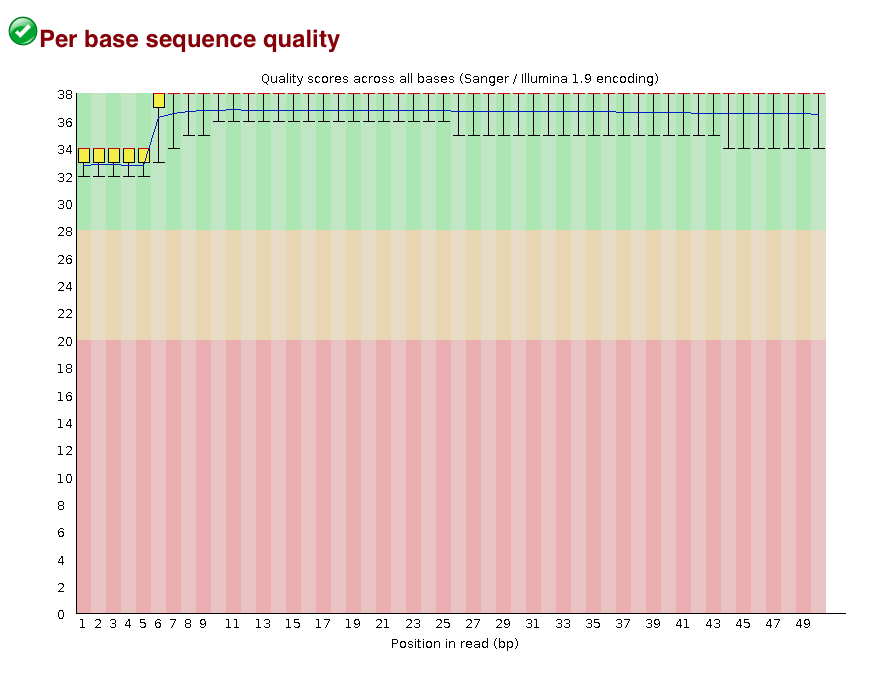
\includegraphics{trimmedNs_negative_fastqc.png}\\

\href{/d/projects/u/sj003/course_materials/fastq/coursework_1/trimmedNs_Negative_fastqc.html}{fastqc
report trimmed}

\emph{b) Use bowtie2 to align the reads to reference genome using two
different options.}

To align both the original file and the trimmed file using bowtie2
against the reference genome, AFPN02.1, and generate a .sam file to use
for further analysis:

\begin{Shaded}
\begin{Highlighting}[]
\BuiltInTok{time}\NormalTok{ /s/software/anaconda/python3/bin/bowtie2 --end-to-end -x }\VariableTok{$\{st_path\}}\NormalTok{/course_materials/genomes/AFPN02.1/AFPN02.1_merge -q }\VariableTok{$\{st_path\}}\NormalTok{/course_materials/fastq/trimmed_Negative.fq -S Negative.sam }\OperatorTok{2>}\NormalTok{ Negative_bowtie_stats.txt}
\end{Highlighting}
\end{Shaded}

\begin{Shaded}
\begin{Highlighting}[]
\BuiltInTok{time}\NormalTok{ /s/software/anaconda/python3/bin/bowtie2 --end-to-end -x }\VariableTok{$\{st_path\}}\NormalTok{/course_materials/genomes/AFPN02.1/AFPN02.1_merge -q }\VariableTok{$\{st_path\}}\NormalTok{/course_materials/fastq/trimmedNs_Negative.fq -S Negative2.sam }\OperatorTok{2>}\NormalTok{ Negative2_bowtie_stats.txt}
\end{Highlighting}
\end{Shaded}

The text file can be examined on the bash terminal, and the .sam file
can be analysed in a multiqc display showing that the new Negative
alignment (Negative2) has the same stats as Positive:

\begin{Shaded}
\begin{Highlighting}[]
\ExtensionTok{/s/software/anaconda/python3/bin/multiqc}\NormalTok{ . -f}
\end{Highlighting}
\end{Shaded}

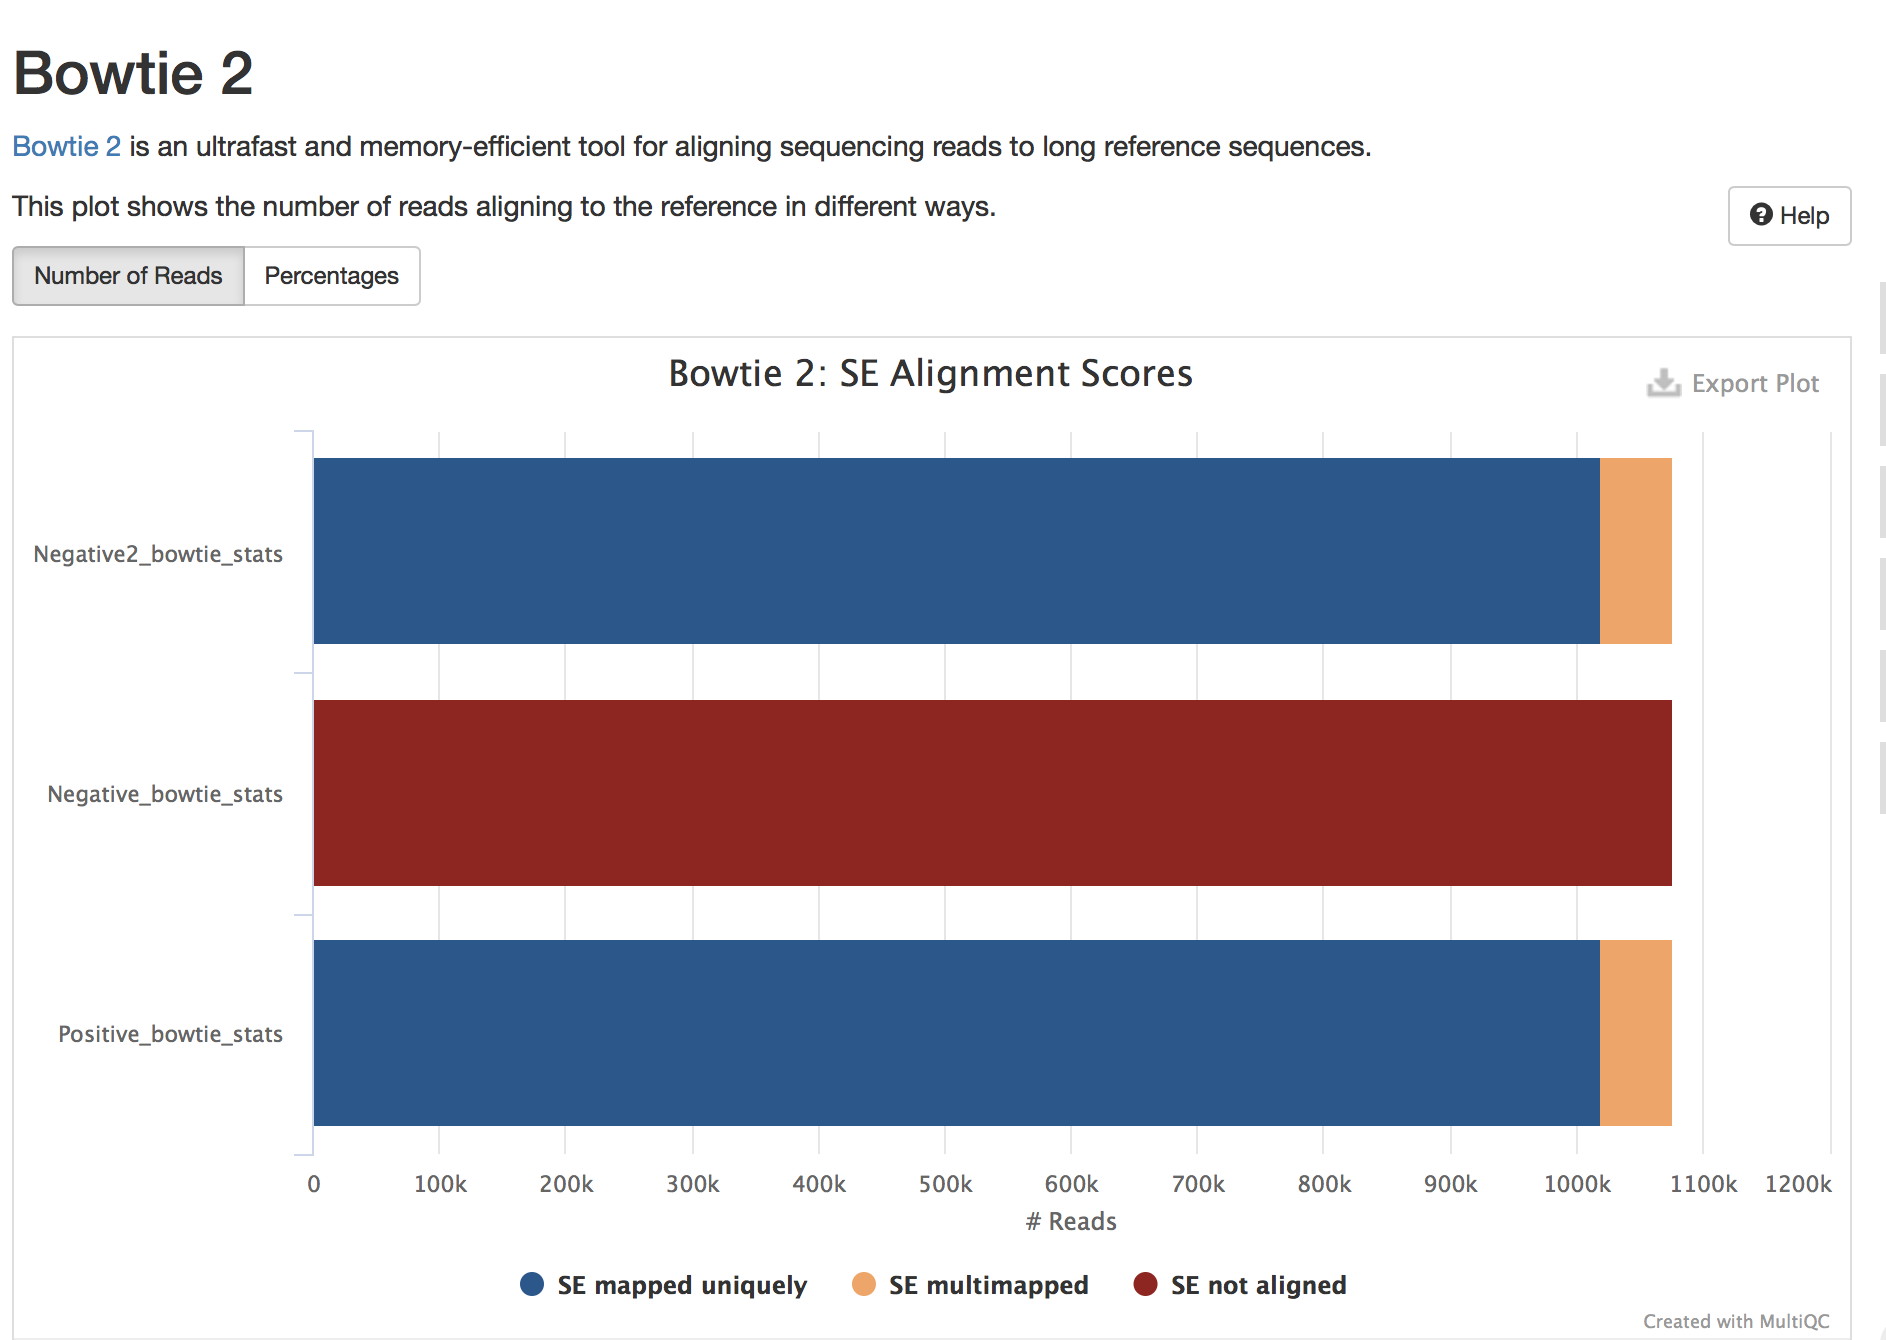
\includegraphics{Neg_v_Pos_multiq.png}\\

Another option is to align the Negative file using options in Bowtie2
that ignore the first and last bases when aligning:

\begin{Shaded}
\begin{Highlighting}[]
\BuiltInTok{time}\NormalTok{ /s/software/anaconda/python3/bin/bowtie2 --end-to-end --trim5 5 --trim3 4 -x }\VariableTok{$\{st_path\}}\NormalTok{/course_materials/genomes/AFPN02.1/AFPN02.1_merge -q }\VariableTok{$\{st_path\}}\NormalTok{/course_materials/fastq/trimmed_Negative.fq -S Negative3.sam }\OperatorTok{2>}\NormalTok{ Negative3_bowtie_stats.txt}
\end{Highlighting}
\end{Shaded}

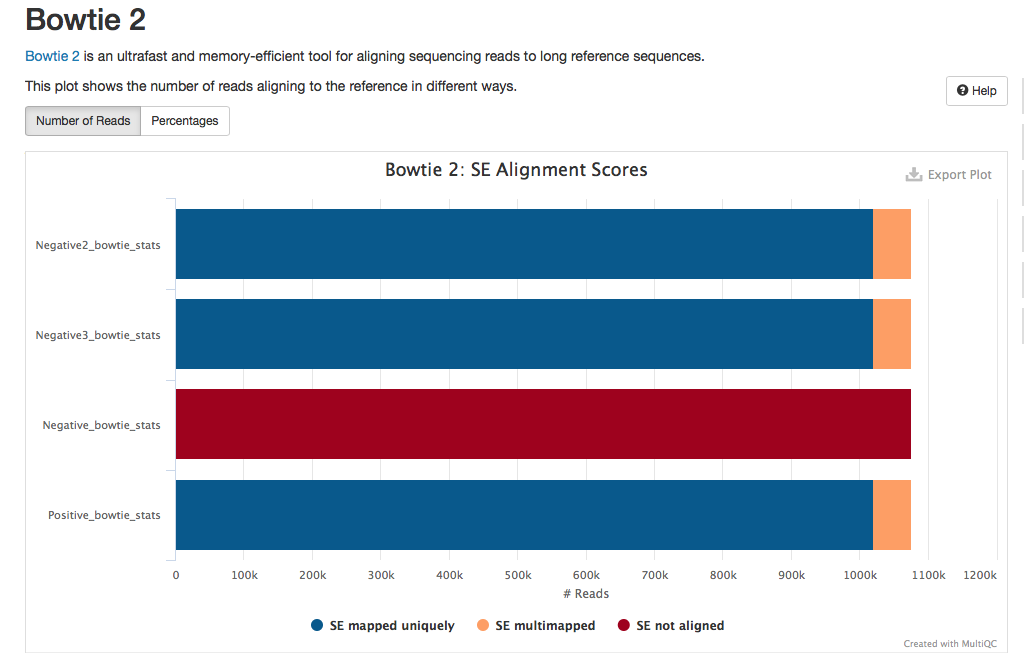
\includegraphics{cw1_q1_multiqc.png}\\
This gives the same alignment results as using cutadapt.

I can also try a local alignment on the file where I cut the Ns off to
see if this improves the alignment:

\begin{Shaded}
\begin{Highlighting}[]
\BuiltInTok{time}\NormalTok{ /s/software/anaconda/python3/bin/bowtie2 --local -x }\VariableTok{$\{st_path\}}\NormalTok{/course_materials/genomes/AFPN02.1/AFPN02.1_merge -q }\VariableTok{$\{st_path\}}\NormalTok{/course_materials/fastq/trimmedNs_Negative.fq -S Negative4.sam }\OperatorTok{2>}\NormalTok{ Negative4_bowtie_stats.txt}
\end{Highlighting}
\end{Shaded}

\begin{enumerate}
\def\labelenumi{\alph{enumi})}
\setcounter{enumi}{2}
\tightlist
\item
  samtools stats:
\end{enumerate}

Negative.sam original

Negative2.sam trimmed Ns with cutadapt

Negative3.sam aligned with trimming Ns with bowtie

Negative4.sam local alignment

In order to save time running samtools for each file, I wrote a bash
script (d/projects/u/sj003/results\_cw1/samtools\_bash.sh)

\begin{Shaded}
\begin{Highlighting}[]
\CommentTok{#!/bin/bash}
\CommentTok{# samtools_bash.sh}
\CommentTok{# script to run basic samtools functions for each file in folder:}

\CommentTok{# Assign everything ending in .sam to SAMFILES variable}
\VariableTok{SAMFILES=}\ExtensionTok{*.sam}

\CommentTok{# Loop over SAMFILES and run samtools for each file}
\KeywordTok{for} \FunctionTok{file}\NormalTok{ in }\VariableTok{$SAMFILES}
\KeywordTok{do}
  \VariableTok{filename=$(}\FunctionTok{basename} \StringTok{"}\VariableTok{$file}\StringTok{"}\VariableTok{)}
  \VariableTok{filename=}\StringTok{"}\VariableTok{$\{filename%}\NormalTok{.*}\VariableTok{\}}\StringTok{"}
  
  \BuiltInTok{echo} \StringTok{"Sort file:        }\VariableTok{$file}\StringTok{"}
  \BuiltInTok{echo} \StringTok{"Index file:       }\VariableTok{$filename}\StringTok{.bam"}
  \BuiltInTok{echo} \StringTok{"Create stats for file:        }\VariableTok{$file}\StringTok{"}
  \BuiltInTok{echo} \StringTok{"Create flagstat for file:       }\VariableTok{$file}\StringTok{"}

  \CommentTok{#Call samtools functions for each file}
  \ExtensionTok{/s/software/samtools/v1.9/bin/samtools}\NormalTok{ sort }\VariableTok{$\{file\}} \OperatorTok{>} \VariableTok{$\{filename\}}\NormalTok{.bam}
  \ExtensionTok{/s/software/samtools/v1.9/bin/samtools}\NormalTok{ index }\VariableTok{$\{filename\}}\NormalTok{.bam}
  \ExtensionTok{/s/software/samtools/v1.9/bin/samtools}\NormalTok{ stats }\VariableTok{$\{file\}} \OperatorTok{>} \VariableTok{$\{filename\}}\NormalTok{_stats.txt}
  \ExtensionTok{/s/software/samtools/v1.9/bin/samtools}\NormalTok{ flagstat }\VariableTok{$\{file\}} \OperatorTok{>} \VariableTok{$\{filename\}}\NormalTok{_flagstat.txt}

  \BuiltInTok{echo}\NormalTok{ -e }\StringTok{"######################\textbackslash{}n\textbackslash{}n"}
\KeywordTok{done}
\end{Highlighting}
\end{Shaded}

Call the script using:

\begin{Shaded}
\begin{Highlighting}[]
\FunctionTok{bash}\NormalTok{ samtools_bash.sh}
\end{Highlighting}
\end{Shaded}

Run a MultiQC report to summarise the sequence and alignment data for
all the alignments.

\begin{Shaded}
\begin{Highlighting}[]
\ExtensionTok{/s/software/anaconda/python3/bin/multiqc}\NormalTok{ . -n q1_multiqc_report}
\end{Highlighting}
\end{Shaded}

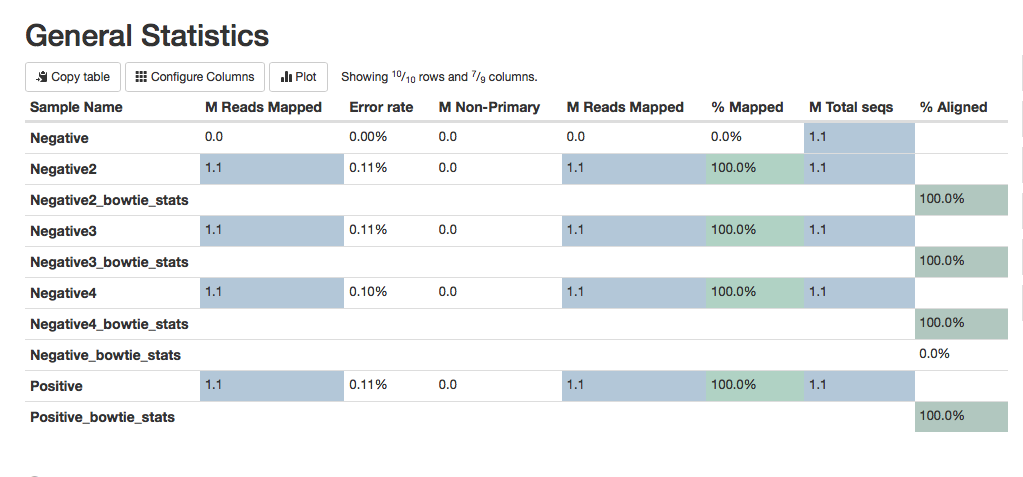
\includegraphics{MultiQCstats_Q1.png}\\
\href{/d/projects/u/sj003/results_cw1/q1_multiqc_report.html}{multiq
report}

The report shows that the best quality alignment is for the local
alignment of the sequences that had the 5' and 3' N's cut off using
cutadapt (Negative4). This alignment had a slightly better error rate
(0.10\%) than the Positive alignment (which was done using the
end-to-end alignmnent), or the edited Negative sequence using the
end-to-end alignment. The local alignment allows some of the bases on
the ends to be omitted to get a better alignment score. It basically
just skips a base at the beginning or end if it doesn't align, and that
may account for the very slightly better error rater. All 1.1M reads
were mapped. I think it is a better idea to edit the N's out of the
sequence reads at the outset, using cutadapt, rather than to just ignore
them using the settings in bowtie2. This way the fastqc reports will
accurately represent the overall sequence quality and the sequence reads
can be used in other software applications without further adjustment.

\subsection{Question 2}\label{question-2}

\emph{Use cutadapt to re-process the BQ.fq file and bowtie2 to map reads
to reference genome. Discuss trade-off between improved mapping rate and
error rate. Which is more important considering goal of coming up with
most accurate genomic reference sequence for sampled bacterium?}

The first step is to examine the fasta file for the BQ sequence reads.
Similar to Negative sequences above, they contain 5' and 3' Ns that need
to be trimmed before alignment can occur. Using cutadapt, this can be
accomplished the same way as we did in question 1:

\begin{Shaded}
\begin{Highlighting}[]
\ExtensionTok{/s/software/anaconda/python3/bin/cutadapt}\NormalTok{ --trim-n -o trimmedns_BQ.fq trimmed_BQ.fq}
\FunctionTok{less}\NormalTok{ trimmedNs_negative.fq}
\end{Highlighting}
\end{Shaded}

We can examine the fastqc report of the edited sequence:

\begin{Shaded}
\begin{Highlighting}[]
\ExtensionTok{/s/software/fastqc/v0.11.8/FastQC/fastqc}\NormalTok{ trimmedns_BQ.fq}
\end{Highlighting}
\end{Shaded}

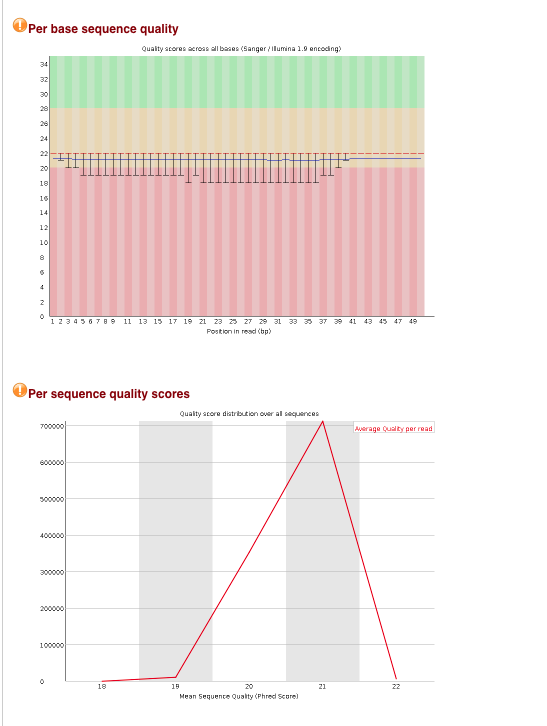
\includegraphics{trimmedns_BQ_fastqc.png}\\

This shows that though the quality of the ends is no longer as poor, the
entire sequence has rather low sequence quality, with an average Phred
score of 21.

Looking at the alignment of BQ with the bacterial genome reference
sequence, we can see the mapping statistics are rather poor at an
overall alignment rate of 82.82\%:

\begin{Shaded}
\begin{Highlighting}[]
\BuiltInTok{time}\NormalTok{ /s/software/anaconda/python3/bin/bowtie2 --end-to-end -x }\VariableTok{$\{st_path\}}\NormalTok{/course_materials/genomes/AFPN02.1/AFPN02.1_merge -q }\VariableTok{$\{st_path\}}\NormalTok{/course_materials/fastq/trimmedns_BQ.fq -S trimmednsBQ.sam }\OperatorTok{2>}\NormalTok{ trimmednsBQ_bowtie_stats.txt}
\FunctionTok{less}\NormalTok{ trimmednsBQ_bowtie_stats.txt}
\end{Highlighting}
\end{Shaded}

I also performed bowtie2 alignment with the `very sensitive local'
setting to increase the alignment sensitivity and hopefully reduce the
error rate (using local alignment) at the same time, which brings the
overall alignment rate up to 89.43\%.

\begin{Shaded}
\begin{Highlighting}[]
\BuiltInTok{time}\NormalTok{ /s/software/anaconda/python3/bin/bowtie2 --very-sensitive-local -x }\VariableTok{$\{st_path\}}\NormalTok{/course_materials/genomes/AFPN02.1/AFPN02.1_merge -q }\VariableTok{$\{st_path\}}\NormalTok{/course_materials/fastq/trimmedns_BQ.fq -S trimmednsBQ_vsl.sam }\OperatorTok{2>}\NormalTok{ trimmednsBQvsl_bowtie_stats.txt}
\FunctionTok{less}\NormalTok{ trimmednsBQvsl_bowtie_stats.txt}
\end{Highlighting}
\end{Shaded}

The `very sensitive' setting has preset parameters that are designed to
maximise sensitivity and accuracy. However, you can manually adjust
these parameters, for example changing the the number of mismatches
permitted per `seed' in the alignment (using -N). I tried changing this
parameter to 0, but using the same settings for the rest of the
parameters as the very-sensitive-local setting uses (-D 20 -R 3 -N 1 -L
20 -i S,1,0.50). This increases the overall alignment rate to 98.64\%
but at what cost to the error rate?

\begin{Shaded}
\begin{Highlighting}[]
\BuiltInTok{time}\NormalTok{ /s/software/anaconda/python3/bin/bowtie2 --local -D 20 -R 3 -N 1 -L 20 -i S,1,0.50 -x }\VariableTok{$\{st_path\}}\NormalTok{/course_materials/genomes/AFPN02.1/AFPN02.1_merge -q }\VariableTok{$\{st_path\}}\NormalTok{/course_materials/fastq/trimmedns_BQ.fq -S trimmednsBQ_cust.sam }\OperatorTok{2>}\NormalTok{ trimmednsBQcust_bowtie_stats.txt}
\FunctionTok{less}\NormalTok{ trimmednsBQcust_bowtie_stats.txt}
\end{Highlighting}
\end{Shaded}

To evaluate the statistics for the alignments, I will call the samtools
script to run the samtools functions for these files.

\begin{Shaded}
\begin{Highlighting}[]
\FunctionTok{bash}\NormalTok{ samtools_bash.sh}
\end{Highlighting}
\end{Shaded}

Run a MultiQC report to summarise the sequence and alignment data for
all the alignments.

\begin{Shaded}
\begin{Highlighting}[]
\ExtensionTok{/s/software/anaconda/python3/bin/multiqc}\NormalTok{ . -f -n q2_multiqc_report}
\end{Highlighting}
\end{Shaded}

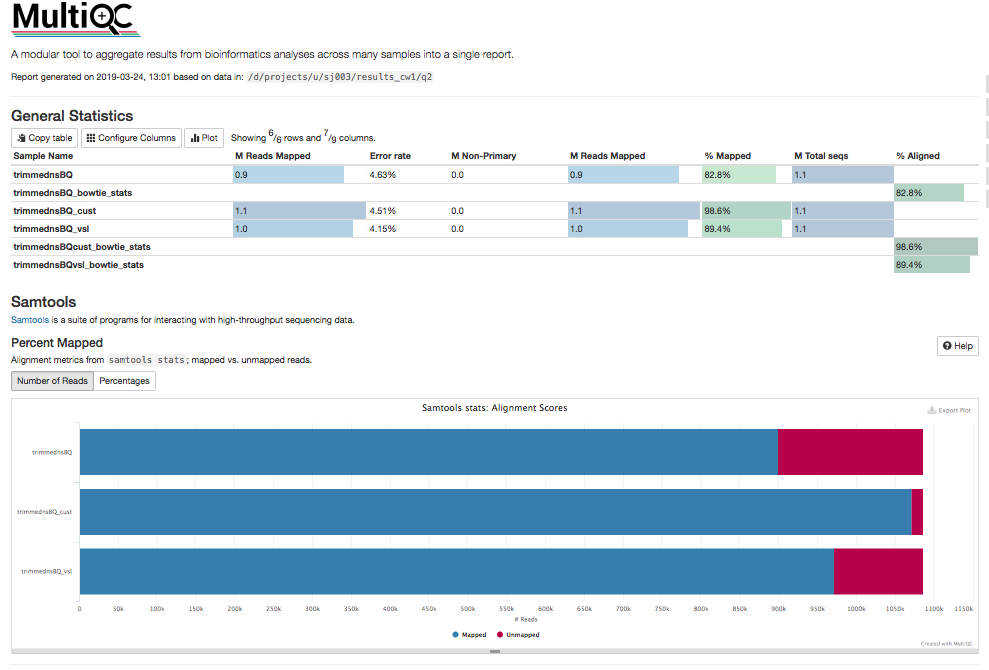
\includegraphics{Multiqc_report_q2.png}\\
\href{/d/projects/u/sj003/results_cw1/q2_multiqc_report.html}{multiqc
report}

\begin{longtable}[]{@{}lll@{}}
\toprule
Sequence & MReads mapped/\% & Error Rate\tabularnewline
\midrule
\endhead
trimmednsBQ & 0.9 / 82.8\% & 4.63\%\tabularnewline
trimmednsBQ\_vsl & 1.0 / 89.4\% & 4.15\%\tabularnewline
trimmednsBQ\_cust & 1.1 / 98.6\% & 4.51\%\tabularnewline
\bottomrule
\end{longtable}

The report shows that there is a trade-off between alignment rate and
error rate. To achieve the best alignment percentage, we have to accept
an error rate of 4.51\% using the custom parameters (trimmednsBQ\_cust).
The next best alignment rate, using the very sensitive local parameters
(trimmednsBQ\_vsl) has a lower error rate of 4.15\%. While this is
better, I am not sure if any error rate above 4\% is acceptable for a
consensus genome. Perhaps the sequencing runs should be repeated to try
to get more high quality sequences.

\subsection{Question 3}\label{question-3}

\emph{Split the BQ aligned files into SAM files containing subsets of
the full set of aligned reads.}

\emph{Split into:}

\emph{a) one file containing multimapping reads and another file with
only uniquely mapped reads}

\begin{Shaded}
\begin{Highlighting}[]
\CommentTok{# for uniquely mapped reads (with MAPQ < 10); all other files in multiBQ file (-U)}
\ExtensionTok{/s/software/samtools/v1.9/bin/samtools}\NormalTok{ view -bq 10 trimmednsBQ.bam }\OperatorTok{>}\NormalTok{ uniqueBQ.bam -U multiBQ.bam}
\end{Highlighting}
\end{Shaded}

\emph{b) one file with unmapped reads and one with only mapped reads}

\begin{Shaded}
\begin{Highlighting}[]
\CommentTok{# includes unique reads (removes unmapped reads with flag of [4])}
\ExtensionTok{/s/software/samtools/v1.9/bin/samtools}\NormalTok{ view -bF 4 trimmednsBQ.bam }\OperatorTok{>}\NormalTok{ mappedBQ.bam}

\CommentTok{# includes only unmapped reads (with flag [4])}
\ExtensionTok{/s/software/samtools/v1.9/bin/samtools}\NormalTok{ view -bf 4 trimmednsBQ.bam }\OperatorTok{>}\NormalTok{ unmappedBQ.bam}
\end{Highlighting}
\end{Shaded}

\emph{c) How can output from b be obtained using Bowtie2 instead?}

Using bowtie2 -k option allows us to report the sequences with the
desired number of alignments, which in this case I am using 1 to get
reads that have only matched once. Unfortunately, this leaves the
unaligned sequences in the file. Looking for solutions online, it seems
there was a different command in bowtie (versus bowtie2), -m, that was
able to filter by number of hits. Looking online, all the advice seems
to be that the most logical thing is to do this using the flags in
samtools, like I've done in b.

\begin{Shaded}
\begin{Highlighting}[]
\CommentTok{## filters for only unique reads (-k) but still contains unaligned seqs}
\BuiltInTok{time}\NormalTok{ /s/software/anaconda/python3/bin/bowtie2 --end-to-end -k 1 -x }\VariableTok{$\{st_path\}}\NormalTok{/course_materials/genomes/AFPN02.1/AFPN02.1_merge -q }\VariableTok{$\{st_path\}}\NormalTok{/course_materials/fastq/trimmedns_BQ.fq -S trimmednsBQ2.sam }\OperatorTok{2>}\NormalTok{ trimmednsBQ2_stats.txt}
\end{Highlighting}
\end{Shaded}

\emph{d) Use BLAST to identify origin of unmapped reads.} To do this, I
used samtools fasta function to convert from a .bam file to a fasta
file.

\begin{Shaded}
\begin{Highlighting}[]
\ExtensionTok{/s/software/samtools/v1.9/bin/samtools}\NormalTok{ fasta unmappedBQ.bam }\OperatorTok{>}\NormalTok{ unmappedBQ.fa}
\end{Highlighting}
\end{Shaded}

Then I cut and pasted 10 sequences from the fasta file into blastn
window and searched on the nr/nt nucleotide database to evaluate the
origin of the sequences. For 9 of the sequences Homo sapiens was the top
hit, and for one of them, Pan troglodytes was the top hit (chimpanzee).
I am assuming there was some contamination of the e coli sample by human
DNA during purification or library construction. None of these 10 were e
coli sequences.

\href{https://blast.ncbi.nlm.nih.gov}{blastn website}

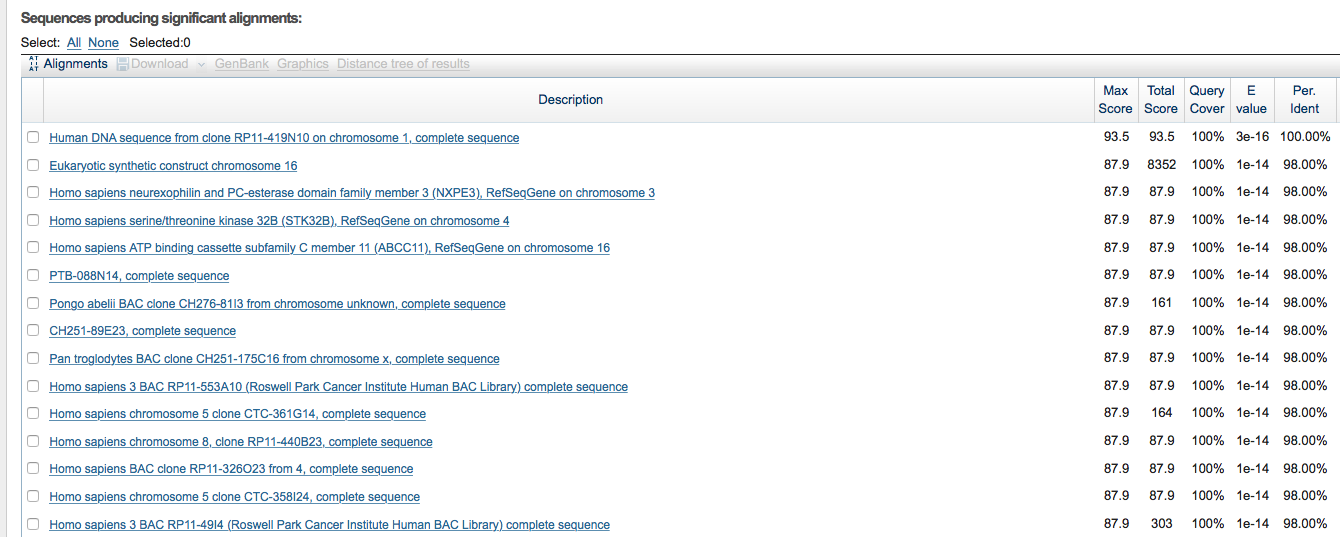
\includegraphics[width=0.75000\textwidth]{blast.png}\\


\end{document}
